\chapter{Problema}
\label{chap:problema}

\section{Introduzione} \label{sec:problemaIntroduzione}
Bitcoin è a tutti gli effetti una criptovaluta pseudo-anonima, questa sua caratteristica all’inizio ha suscitato particolare interesse all’interno del \emph{Dark Web}; diventando nel 2011 la moneta principale utilizzata per attività come il riciclaggio di denaro, incluse molte attività nel mercato nero. \\
Il concetto di distributed ledger associato all’utilizzo estensivo di Bitcoin per attività illecite, ha dato vita a numerosi studi di analisi forense per tracciare il flusso del denaro. \\
Il \emph{tracking} del flusso di bitcoin nella maggior parte dei casi viene effettuato tramite la creazione di grafi con cui eseguire le opportune analisi. \\
I grafi più comuni utilizzati sono i grafi di transazioni e i grafi degli address.

\section{Grafo delle transazioni} \label{sec:grafoDelleTransazioniProblema}
Attraverso l’introduzione dei concetti basilari della tecnologia Bitcoin (Capitolo \ref{chap:bitcoin}) la creazione di questo grafo risulta quasi intuitiva, infatti si può ricostruire il flusso delle transazioni utilizzando il backlink contenuto all’interno delle transazioni di input.
Riesaminando l’Esempio \ref{example:aliceBobFirst}, possiamo costruire un grafo delle transazioni coinvolte nello scambio di bitcoin tra Alice e Bob: quando abbiamo esaminato la nuova transazione prodotta da Alice e indirizzata a Bob con l’id \say{ddd587d\-54b693\-a9bc9bda\-2218c6f5e17\-979f6ac53755\-c5c1f668f3fa\-728e472d} abbiamo osservato che all’interno della transazione di input era contenuto un id di transazione appartenente ad un precendete UTXO in possesso di Alice che ricordiamo essere: \say{a57c2a4\-27dfa\-591b1243\-343c8413\-c249faac\-3e5df2fe\-4fa1fc93dca\-3d904f3c7}. \\ %Abbiamo messo accapo
In Figura \ref{fig:graphtxproblem} viene rappresentato il grafo risultante.

{\centering
\vspace{5pt}
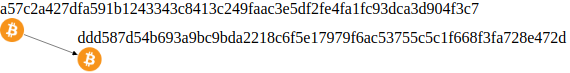
\includegraphics[scale=0.35]{images/exampleWithGraph/aliceBoxTx.png}
\captionof{figure}{Rappresentazione sotto forma di grafo della transazione tra Alice e Bob descritta nell’Esempio \ref{example:aliceBobFirst}.\label{fig:graphtxproblem}}
\vspace{10pt}
\par}

\section{Grafo degli address} \label{sec:grafoDegliAddressProblema}
La creazione di questa tipologia di grafo è molto meno intuitiva, perché come visto nel Capitolo \ref{chap:bitcoin}, la tecnologia non utilizza nessun riferimento a wallet o persone, ma basterebbe una chiave privata con la rispettiva chiave pubblica per interagire con l’intero sistema. \\
Gli address generati attraverso la chiave pubblica sono contenuti all’interno dello script di blocco in modo da rendere la transazione sbloccabile solo dal proprietario dell’address. \\
Come descritto nella Sezione \ref{sec:bitcoinScriptBitcoin}, gli address possono essere originati anche da uno script tipo P2SH, P2WPKH e P2WSH; ciò rende la creazione del grafo degli address molto insidiosa, perché gli address ricavati dagli script (se utilizzati correttamente) sono univoci e quindi rappresenterebbero un’identità diversa all’interno del grafo, anche se molti di questi potrebbero appartenere allo stesso wallet. \\
Come illustrato nell’Esempio \ref{example:aliceBobFirst} Alice genera una nuova transazione consumando un suo UTXO con un valore maggiore o uguale del valore di bitcoin necessario; nell'esempio viene utilizzato un UTXO con un quantitativo maggiore, comportando così la generazione di una exchange transaction. \\
Questo tipo di transazione porta alle seguenti riflessioni:

\begin{itemize}
  \item L’exchange transaction potrebbe contenere un address differente, in questo specifico caso la transazione contiene un address ricavato da uno script Witness (che potrebbe essere ricavato dalla medesima chiave pubblica o da chiavi pubbliche distinte contenute all’interno del wallet).

  \item L'exchange transaction potrebbe contenere uno script P2PKH e quindi un indirizzo primitivo, ma quest’ultimo potrebbe essere differente dall’address di origine. Questo lascerebbe pensare che i bitcoin si siano diretti verso un nuovo proprietario.
  Nella maggior parte dei casi è solo una tecnica per aumentare la privacy utilizzata dai wallet.
  Ad oggi molti dei wallet utilizzati contengono un set di chiavi private che permette loro di generare un address diverso ad ogni nuova operazione.
\end{itemize}

La creazione del grafo contiene quindi una serie di problematiche riguardante gli address, che possiamo riassumere in:

\begin{itemize}
  \item Il destinatario potrebbe usare indirizzi originati da script (come un address P2SH) rendendo così difficile associare l’appartenenza allo stesso wallet di più address; oppure l’address potrebbe camuffare uno script P2MS N:M con destinatari distinti. \\
  In Figura \ref{fig:alicebobgraphaddress} viene rappresentato il grafo di address coinvolti nell’Esempio \ref{example:aliceBobFirst}, dove l’address \say{33mMAc6nGyENdKMQTr5SrKoEkwNTeZQUx9} rappresenta una particolare tipologia di indirizzo utilizzato da Bob, infatti l’address viene ricavato da uno script P2WSH che a sua volta camuffa uno script P2MS. \\
  Bob ha infatti utilizzato uno script P2MS con due address differenti al suo interno, appartenenti allo stesso wallet. \\
  Gli address che iniziano per \say{bc1q} appartengono al medesimo wallet di Alice; in cui è presente un exchange transaction (Il modo in cui viene ricavato l’address dalla transazione di input verrà illustrato successivamente).

  {\centering
  \vspace{15pt}
  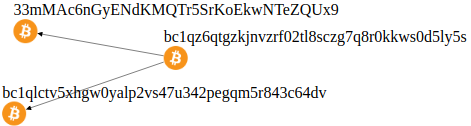
\includegraphics[scale=0.43]{images/exampleWithGraph/exchange-transaction-alice-bob.png}
  \captionof{figure}{Rappresentazione del grafo di address coinvolti nella transazione illustrata nell’Esempio \ref{example:aliceBobFirst}.\label{fig:alicebobgraphaddress}}
  \vspace{10pt}
  \par}

  \item La generazione delle exchange transaction contiene, nella maggior parte dei casi, un address ricavato da una chiave pubblica diversa, appartenente allo stesso wallet.
  \begin{example} \label{example:newalicebobaddress}
   Si consideri un nuovo scenario dove Alice spedisce dei bitcoin a Bob ed entrambi i partecipanti utilizzano address primitivi:  Alice invia all’indirizzo di Bob 0.00336527 bitcoin, generando una nuova transazione con il seguente id \say{8b22a9\-d19ee58ee1b\-5283632f70\-fbeceaf13\-948dbc3d\-48ea22c02\-1a1d82\-e1f06} verso l’address di Bob \say{1CPD7DqguruujwvfaegKsV6ewiFvSZTiB3}.
    Il wallet di Alice utilizza un suo UTXO per per effettuare la spedizione di bitcoin con un valore maggiore del necessario, quindi il wallet è costretto a generare un exchange transaction per dividere UTXO. \\
    L’UTXO di Alice con un valore di bitcoin pari a 0.00682055 bitcoin si frammenta in due nuove transazioni:

    \begin{itemize}
      \item La transazione verso Bob del valore di 0.00336527 bitcoin.
      \item L’exchange transaction verso il wallet di Alice del valore di 0.00341851 bitcoin.
    \end{itemize}

    La Figura \ref{fig:newalicebobaddress} rappresenta il grafo risultante degli address coinvolti.
    {\centering
    \vspace{15pt}
    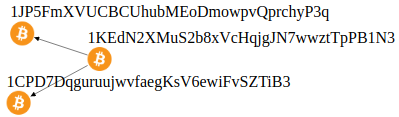
\includegraphics[scale=0.43]{images/exampleWithGraph/example-p2pkh-exchange-transaction.png}
    \captionof{figure}{Rappresentazione del grafo degli address coinvolti nella transazione dell’esempio \ref{example:newalicebobaddress}.\label{fig:newalicebobaddress}}
    \vspace{10pt}
    \par}

    In Figura \ref{fig:newalicebobaddress} si possono osservare tre address distinti originati da chiavi pubbliche distinte, dove però i proprietari sono solo Alice e Bob:
    \begin{itemize}
      \item Gli address di Alice sono: \say{1KE\-dN2XMu\-S2b8xVc\-HqjgJN\-7wwztT\-pPB1N3}, che rappresenta l’address di orgine; \\
      \say{1JP5F\-mXVUCB\-CUhubME\-oDmowpv\-Qprchy\-P3q} che rappresenta l’address a cui viene indirizzata l’exchange transaction. Entrambi gli address appartengono al wallet di Alice ma originate da chiavi pubbliche diverse.
      \item L’address di Bob inviato ad Alice per eseguire la spedizione di Bitcoin: \say{1CPD7Dq\-guruujwvf\-aegKsV6ew\-iFvSZTiB3}.
    \end{itemize}
  \end{example}
\end{itemize}
Inoltre all’origine di Bitcoin, non tutti i wallet contenevano un set di chiavi private e questo comportava la creazone del exchange transactions verso il medesimo address.
\begin{example}
  Prendiamo in esame la transazione con il seguente id \say{15bf\-8b35c\-9210efe7e448\-c5fc6b69b47b3a8\-cac9c148c7cc\-57c65f266\-384d9b8} in cui possiamo osservare la presenza dell’address \say{1EinmJDn\-33yFPGafKu\-Cw2guUqPSMaNKo5v} sia in output che in input.
  La Figura \ref{fig:exchangeaddressrecicle} rappresenta la transazione ricercata attraverso un esploratore blockchain.

  {\centering
  \vspace{15pt}
  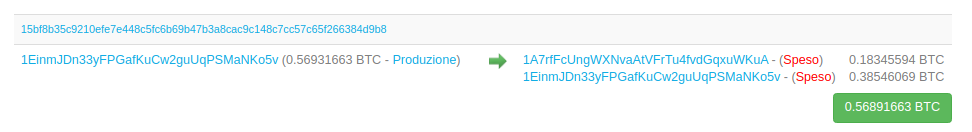
\includegraphics[scale=0.35]{images/exampleWithGraph/exchange-tx-with-same-address.png}
  \captionof{figure}{Rappresenta un exchange transaction verso lo stesso indirizzo di origine\cite{blockstream:esplora}.\label{fig:exchangeaddressrecicle}}
  \vspace{5pt}
  \par}

  In questo caso il flusso di bitcoin è chiaro, La Figura \ref{fig:graphAddresssameaddresschange} rappresenta il grafo di address coinvolti nella transazione.

    {\centering
  \vspace{15pt}
  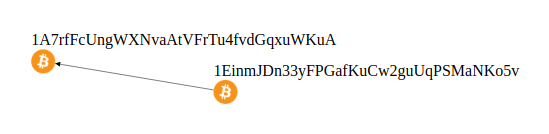
\includegraphics[scale=0.48]{images/exampleWithGraph/exchange-tx-with-same-address-graph.png}
  \captionof{figure}{Rappresenta il grafo risultante degli address coinvolti nella transazione con id 15bf8\-b35c9210\-efe7e448c5fc\-6b69b47b3a\-8cac9c14\-8c7cc57c6\-5f26638\-4d9b8.\label{fig:graphAddresssameaddresschange}}
  \vspace{10pt}
  \par}
\end{example}
La costruzione del grafo oltre ad essere insidiosa per i problemi relativi alla frammentazione degli address, costringe ad accedere alle transazioni di output contenute all’interno delle transazioni, il cui riferimento risiede nelle transazioni di input della nuova transazione, per prelevare l’address di origine.
La Figura \ref{fig:processgetorigin} Illustra il procedimento per ottenere l’address di origine dell’Esempio \ref{example:aliceBobFirst}.

{\vspace{15pt}
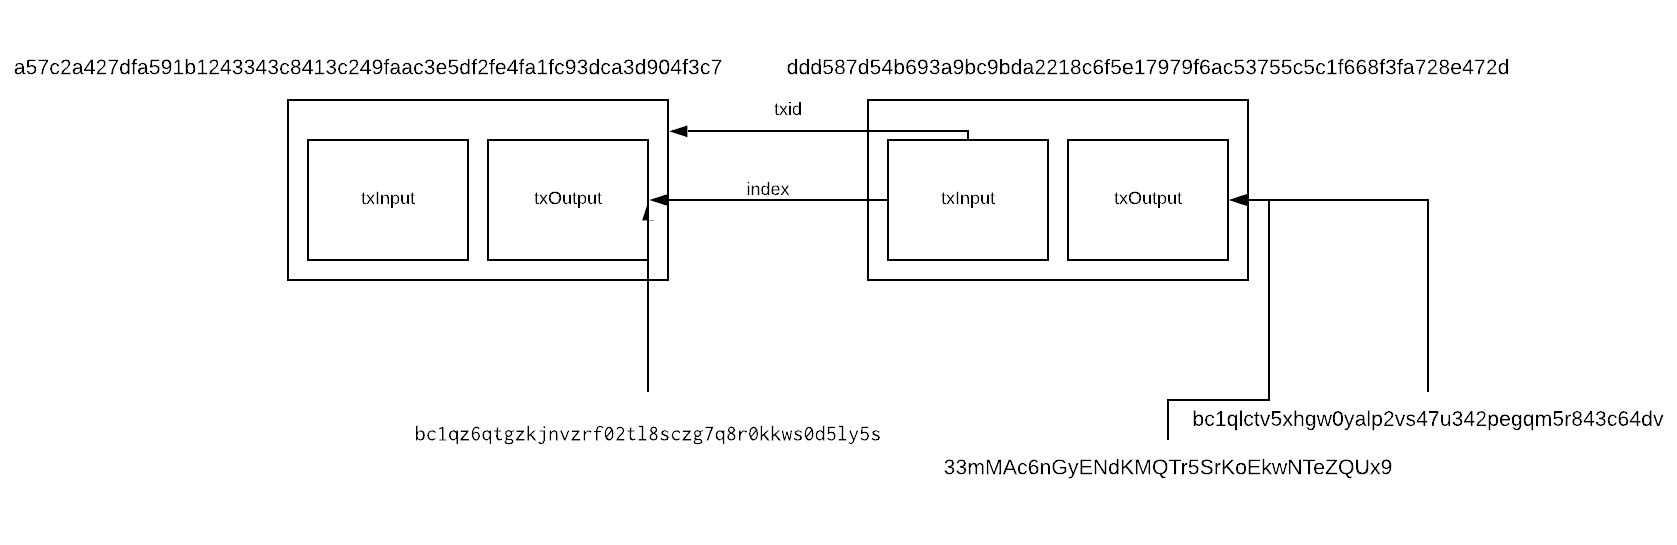
\includegraphics[scale=0.25]{images/howFindTheAddressTo.png}
\captionof{figure}{Rappresentazione del procedimento per determinare l’address di origine.\label{fig:processgetorigin}}
\vspace{10pt}
\par}
